Como enunciamos en la explicaci\'on de nuestro algoritmo, el mismo va chequeando en cada paso si existe alg\'un gimnasio capaz de ser vencido y si existe buscar cual es el m\'as cercano de estos a ser vencidos, por lo tanto existir\'an casos en los cuales la soluci\'on obtenida para los mismos sea la \'optima pero para algunos no lo ser\'a.

Se obtendr\'a la soluci\'on \'optima cuando se reciban pokeparadas y gimnasios en orden, o sea, primero pokeparadas para vencer a un gimnasio cerca de ellas y luego m\'as pokeparadas para vencer a otros gimnasios que se encuentren cerca de estas \'ultimas, se mostrar\'a a continuaci\'on un dibujo que ejemplifica lo dicho:

\vspace*{0.3cm} \vspace*{0.3cm}
  \begin{center}
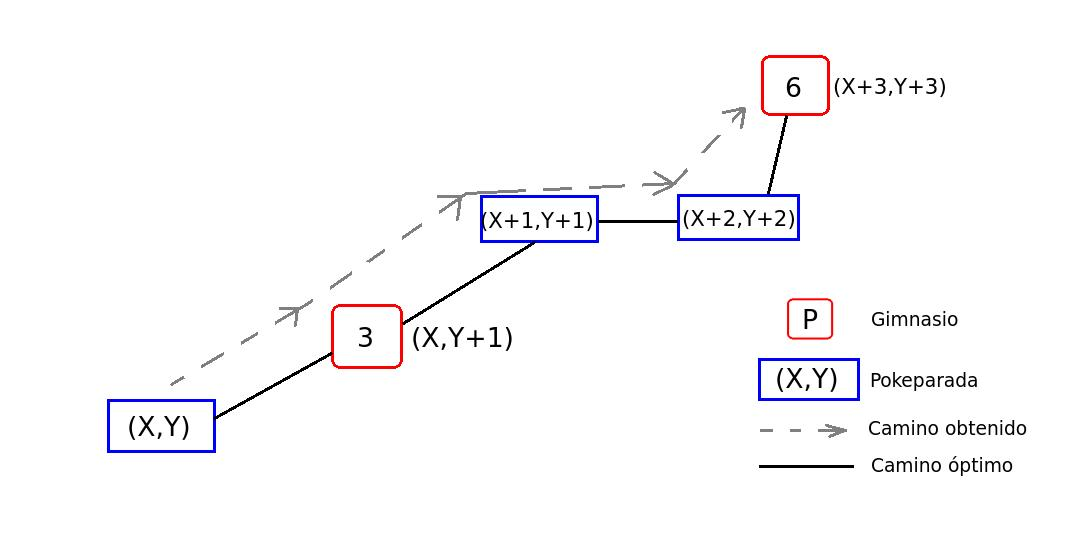
\includegraphics[scale=0.60]{./EJ2/optima.jpeg}
\\{\textit{Ejemplo 2.0 - La soluci\'on obtenida es la \'optima}}
  \end{center}
  \vspace*{0.3cm}

Luego, no se obtendr\'a una soluci\'on \'optima cuando las pokeparadas esten todas juntas y los gimnasios muy lejos, teniendo los gimnasios una cantidad necesaria bastante menor que ciertas sumas de pociones otorgadas por las pokeparadas (TRATAR DE ESCRIBIRLO MEJOR ESTO)

\vspace*{0.3cm} \vspace*{0.3cm}
  \begin{center}
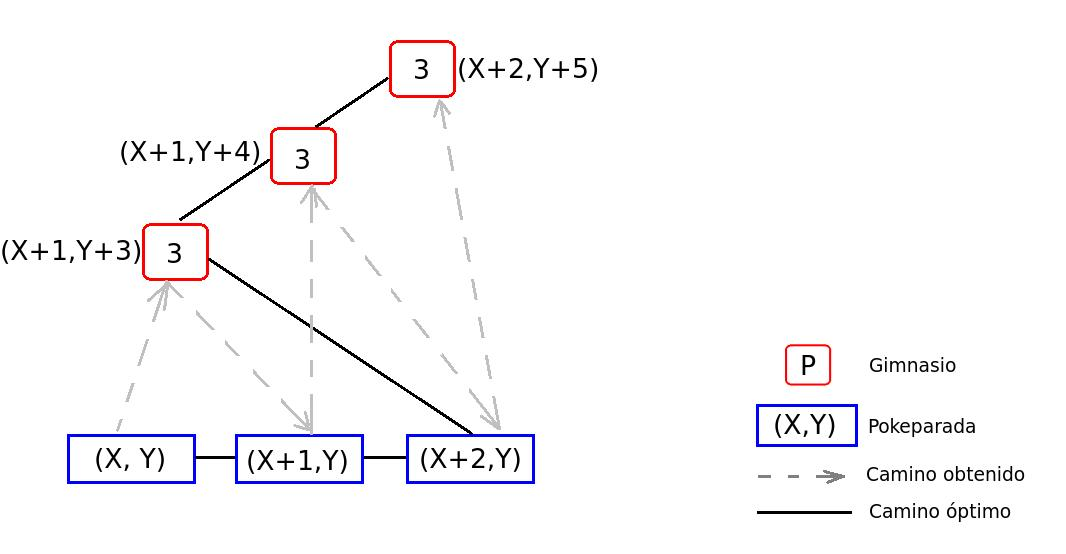
\includegraphics[scale=0.60]{./EJ2/nooptima.jpeg}
\\{\textit{Ejemplo 2.1 La soluci\'on obtenida no es la \'optima}}
  \end{center}
  \vspace*{0.3cm}
  
  
\vspace*{0.3cm} \vspace*{0.3cm}
  \begin{center}
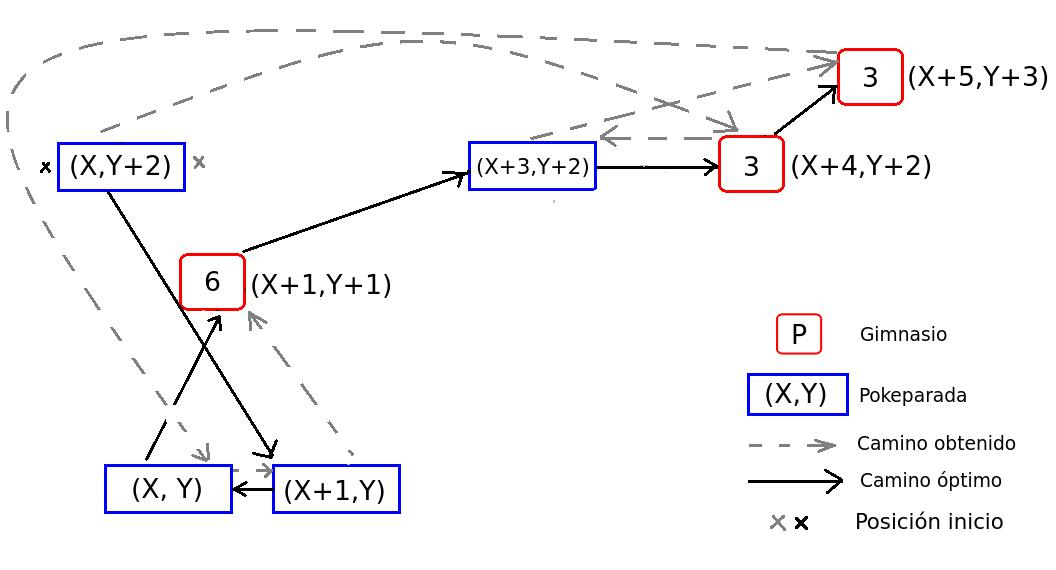
\includegraphics[scale=0.60]{./EJ2/nooptima2.jpeg}
\\{\textit{Ejemplo 2.3 La soluci\'on obtenida no es la \'optima}}
  \end{center}
  \vspace*{0.3cm}

La soluci\'on obtenida que dista de la \'optima puede ser tan mala como la cantidad de veces que se tenga que ir a una pokeparada, ganar gimnasio y luego ir a otra pokeparada a recuperarse por m\'as que esta \'ultima se encuentre mucho m\'as cerca de la pokeparada inicial que el gimnasio.

Se puede observar en el ejemplo 2.1 como nuestro algorimo va a la primer pokeparada y de ah\'i va a vencer al gimnasio mas cercano en vez de ir a la pokeparada que se encuentra inmediatamente consecutiva. Esto lo hace hasta vencer a todos los gimnasios.
Este estilo de caso sera uno de los peores en referencia a la solucion obtenida que se obtenga ya que la misma ser\'a muy distante a la optima
